\documentclass[11pt,a4paper]{article}
\usepackage[utf8]{inputenc}
\usepackage[spanish]{babel}
\usepackage{graphicx}
\usepackage{hyperref}
\usepackage{makecell}
\usepackage{float}

%Opciones de encabezado y pie de página:
\usepackage{fancyhdr}
\pagestyle{fancy}
\lhead{}
\rhead{}
\lfoot{Fundamentos de Redes}
\cfoot{}
\rfoot{\thepage}
\renewcommand{\headrulewidth}{0.4pt}
\renewcommand{\footrulewidth}{0.4pt}

\setlength{\parskip}{10pt}

\begin{document}
	% Pagina de titulo
	\pagenumbering{gobble}

	% Pagina de titulo
	\begin{titlepage}

		\begin{minipage}{\textwidth}

			\centering
			\textsc{\Large Fundamentos de Redes\\[0.2cm]}
			\textsc{GRADO EN INGENIERÍA INFORMÁTICA}\\[1cm]

			\noindent\rule[-1ex]{\textwidth}{1pt}\\[3.5ex]
			{\Huge Práctica 2: Cliente-Servidor\\}
			\noindent\rule[-1ex]{\textwidth}{2pt}\\[3.5ex]
			%{\large\bfseries Ejercicio 5}
		\end{minipage}

		\vspace{1.5cm}
		
		\begin{minipage}{\textwidth}
			\centering

			\textbf{Autores}\\ {Vladislav Nikolov Vasilev\\José María Sánchez Guerrero}\\[2.5ex]

			\vspace{1cm}
			\textsc{Escuela Técnica Superior de Ingenierías Informática y de Telecomunicación}\\
			\vspace{1cm}
			\textsc{Curso 2018-2019}
		\end{minipage}
	\end{titlepage}
	
	%Indice
	\pagenumbering{arabic}
	\tableofcontents
	\newpage
	
	\section{Descripcion de la aplicación}
	La aplicación que se ha desarrollado es \textit{Ahorcado}, inspirada en el popular juego homónimo en el que un jugador tiene que intentar adivinar una palabra en un número máximo de intentos. La aplicación creada sigue el paradigma cliente-servidor, y permite a varios jugadores jugar de forma concurrente. La aplicación permite tanto jugar una o varias partidas como consultar un ránking para ver lo que han tardado otros jugadores en adivinar sus palabras.\par
	En esta versión el jugador dispone de 10 vidas y se le resta una por cada fallo. Si ya ha dicho una letra errónea y la repite después no será penalizado. Además de eso, después de decir la primera letra, el jugador tiene un margen de tiempo de 60 segundos para adivinar la palabra. Si no lo hace en el tiempo dado o si pierde todas las vidas, perderá. En caso de adivinar la palabra, se le pedirá su nombre y se guardará el tiempo que ha tardado, su nombre y la palabra en el ránking.\par
	La aplicación utiliza internamente el protocolo TCP, ya que no interesa que se pueda perder la información al enviar mensajes entre clientes y el servidor.
	
	\section{Diagrama de estados del servidor}
	
	\begin{figure}[H]
	\centering
	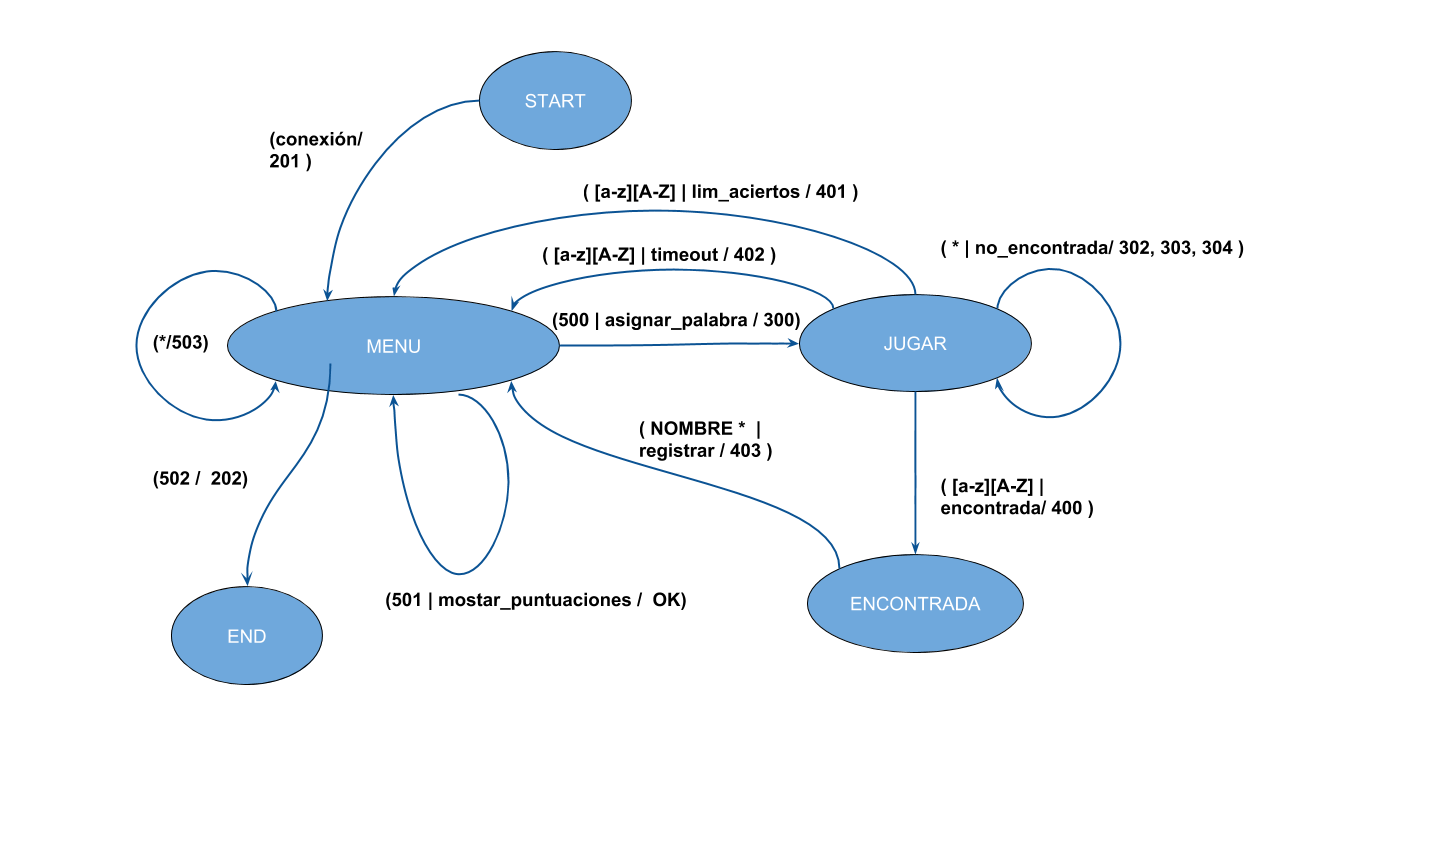
\includegraphics[width=1.2\textwidth]{./EsquemaFR.png}
	\end{figure}	
	
	\section{Mensajes}
		\subsection{Servidor}
		\begin{center}
		\begin{tabular}{| c | c | c |}
		\hline
		\textbf{Código} & \textbf{Cuerpo} & \textbf{Descripción}\\ \hline
		300 & \makecell{``Palabra de \textit{X} letras.\\Tienes \textit{Y} intentos y\\ \textit{T} segundos."} & \makecell{Mensaje informativo de bienvenida al\\juego.}\\ \hline
		301 & \makecell{``Insertar una letra:"} & \makecell{Petición para que el cliente inserte\\una nueva letra.} \\ \hline
		302 & \makecell{``Ya has dicho la letra \textit{L}.\\Te quedan \textit{Y} intentos\\ y \textit{T} segundos."} & \makecell{Informa que el usuario ya ha dicho la letra.} \\ \hline
		303 & \makecell{``Acertaste, te quedan \textit{Y}\\intentos y \textit{T} segundos."} & Informa al usuario que ha acertado la letra. \\ \hline
		304 & \makecell{``La letra \textit{L} no se encuentra\\en la palabra. Te quedan\\\textit{Y} intentos y \textit{T} segundos."} & \makecell{Informa al usuario que la palabra no contiene\\ la letra especificada.}\\ \hline
		400 & \makecell{``Adivinaste la palabra en\\ \textit{T} segundos. Has ganado!"} & \makecell{Indica al usuario que ha adivinado\\ la palabra en un tiempo \textit{T}.} \\ \hline
		401 & \makecell{``Número de intentos superado.\\La palabra era \textit{P}. Has perdido!"} & \makecell{Indica al usuario que se ha quedado\\ sin intentos y le dice la palabra.}\\ \hline
		402 & \makecell{``Se ha agotado el tiempo:\\partida terminada. La palabra\\ era \textit{P}. Has perdido!"} & \makecell{Indica al usuario que se ha quedado\\ sin tiempo y le dice la palabra.}\\ \hline
		403 & ``Escribe tu nombre:" & \makecell{Solicita al usuario que escriba su nombre\\al adivinar la palabra}\\ \hline
		600 & \makecell{Número de elementos\\del ránking a enviar} & \makecell{Indica el número de elementos del\\ ránking que se van a enviar.} \\ \hline
		601 & \makecell{Posición + Tiempo\\ + Nombre + Palabra} & \makecell{Mensaje que contiene una posición del\\ránking.} \\
		\hline
		\end{tabular}
		\end{center}
		\subsection{Cliente}
		\begin{center}
		\begin{tabular}{| c | c | c |}
		\hline
		\textbf{Código} & \textbf{Cuerpo} & \textbf{Descripción}\\ \hline
		500 & & Solicita al servidor el comienzo de una nueva partida. \\ \hline
		501 & & \makecell{Solicita al servidor la consulta de los ránkings. Se consultan los 10\\ primeros puestos, o si hay menos, los que haya.} \\ \hline
		502 & & Permite salir del menú y de la aplicación.\\ \hline
		503 & & Código de error al no haber escogido una opción válida.\\
		\hline
		\end{tabular}
		\end{center}

	\section{Evaluación de la aplicación}
	
	\begin{figure}[H]
	\centering
	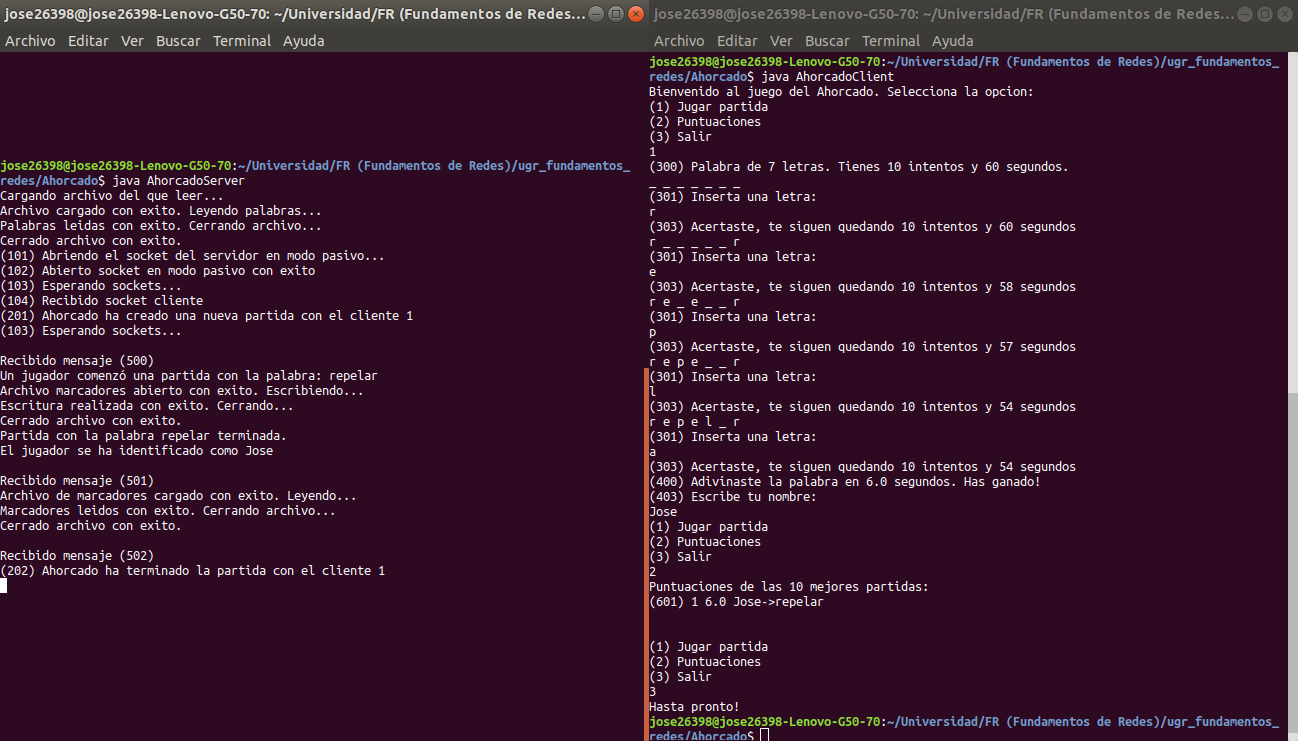
\includegraphics[width=.8\textwidth]{./PartidaNormal.png}
	\caption{Imágen que muestra una partida normal. En la parte izquierda se puede ver el servidor. En la parte derecha, el cliente. El cliente inicia una nueva partida y adivina la palabra. Al acertarla, se le pide insertar el nombre. El jugador inserta su nombre y se guarda el resultado en el archivo de marcadores.} \label{fig:Partida normal}
	\end{figure}
	
	\begin{figure}[H]
	\centering
	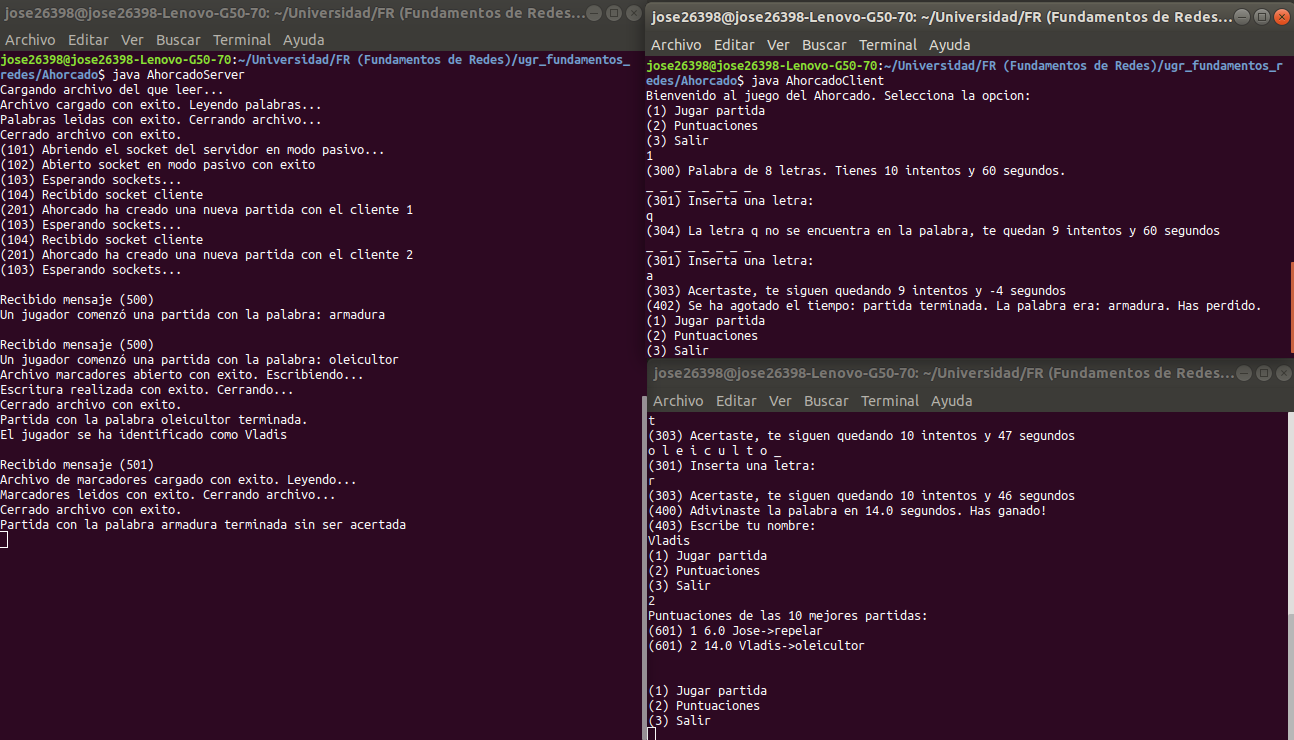
\includegraphics[width=.8\textwidth]{./PartidaConcurrente.png}
	\caption{Imágen que muestra un ejemplo de concurrencia. A la izquierda se ve el servidor, que atiende a más de un cliente concurrentemente. A la derecha se pueden ver 2 clientes. El de arriba había iniciado una partida pero al final ha perdido por quedarse sin tiempo. El de abajo había iniciado una nueva partida y ha acertado la palabra, con lo cuál se le ha pedido su nombre y se ha guardado en los marcadores. A continuación, ha solicidado ver el ránking, con lo cuál se le envía la información solicitada.} \label{fig:Partida concurrente}
	\end{figure}
	
\end{document}